\documentclass[10pt]{beamer}
\usepackage{amsmath}
\usepackage{amssymb}
\usepackage{geometry}
\usepackage{graphicx}
\usepackage{url}
\usepackage{xcolor}

% some latex magic for correcting apostrophe issue in verbatim mode
\makeatletter
\let \@sverbatim \@verbatim
\def \@verbatim {\@sverbatim \verbatimplus}
{\catcode`'=13 \gdef \verbatimplus{\catcode`'=13 \chardef '=13 }} 
\makeatother

\begin{document}
%---------------------------------------------
\begin{frame}
\large
Exam 1 Practice Problems\\
STAT 310, Spring 2021\\
\normalsize
\end{frame}

%---------------------------------------------
\begin{frame}{Exercise 1}
\vspace{-1cm}
The following is a box plot of height in inches for a random sample of people.  Using the box plot, estimate the median and IQR.  Are there any potential outlier in this data set?

\begin{figure}
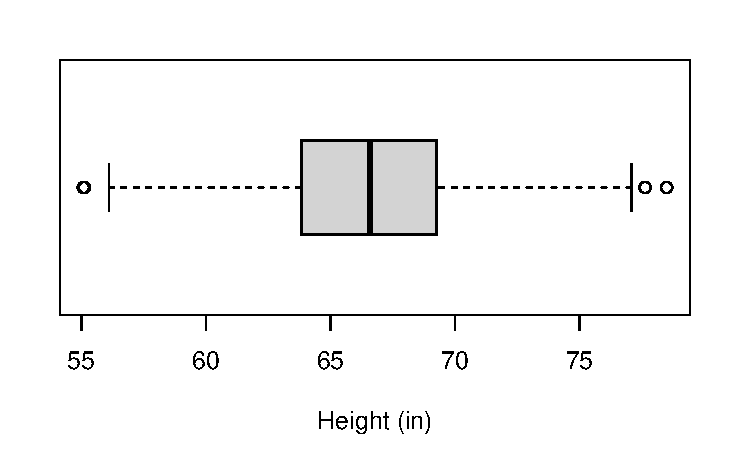
\includegraphics[scale=0.55]{figure/boxplot_height.pdf}
\end{figure}
\end{frame}

%---------------------------------------------
\begin{frame}{Exercise 2}
Describe the shapes of the distributions in the following histograms.

\begin{figure}
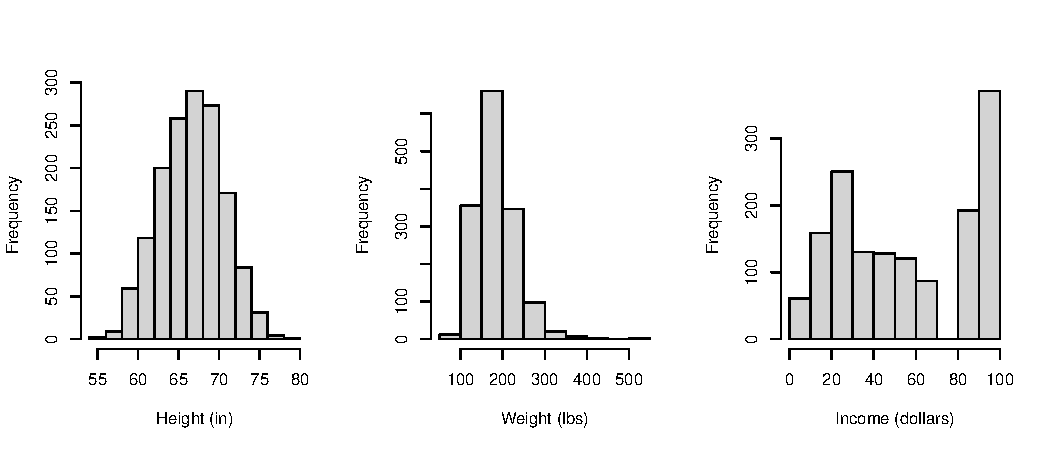
\includegraphics[scale=0.55]{figure/hist3.pdf}
\end{figure}
\end{frame}


%---------------------------------------------
\begin{frame}{Exercise 3}
\vspace{-3cm}
Without doing an calculations, determine whether the mean and standard deviation of Set A is larger than, smaller than, or equal to Set B.  Then use R to verify.\\
\vspace{10pt}
\large
Set A: 1, 2 , 9, 12, 13\\
Set B: 3, 4, 11, 14, 15
\end{frame}

%---------------------------------------------
\begin{frame}{Exercise 4}
\vspace{-3cm}
Without doing an calculations, determine whether the mean and standard deviation of Set A is larger than, smaller than, or equal to Set B.  Then use R to verify.\\
\vspace{10pt}
\large
Set A: 1, 2 , 9, 12, 13\\
Set B: 2, 4, 18, 24, 26\\
\end{frame}

%---------------------------------------------
\begin{frame}{Exercise 5}
Josh, a student in a statistics class, scored 85 points on the first exam and 80 points on the second exam. The mean score on the first exam for all students in this course was 79 with a standard deviation of 4.  The mean score on the second exam was 60 with a standard deviation of 10.  The distributions of both exam scores are approximately normal.
\begin{enumerate}[(a)]
\item What is Josh's $z-$score on the first exam?
\vspace{1cm}
\item What is Josh's $z-$score on the second exam?
\vspace{1cm}
\item On which exam did Josh do better when compared with other students in the class?
\vspace{2cm}
\end{enumerate}
\end{frame}


%---------------------------------------------
\begin{frame}{Exercise 6}
\small
The first histogram 
below shows the distribution of the yearly incomes of 40 patrons at a college 
coffee shop. Suppose two new people walk into the coffee shop: one making 
\$225,000 and the other \$250,000. The second histogram shows the new income 
distribution. Summary statistics are also provided. \\
\begin{minipage}[c]{0.4\textwidth}
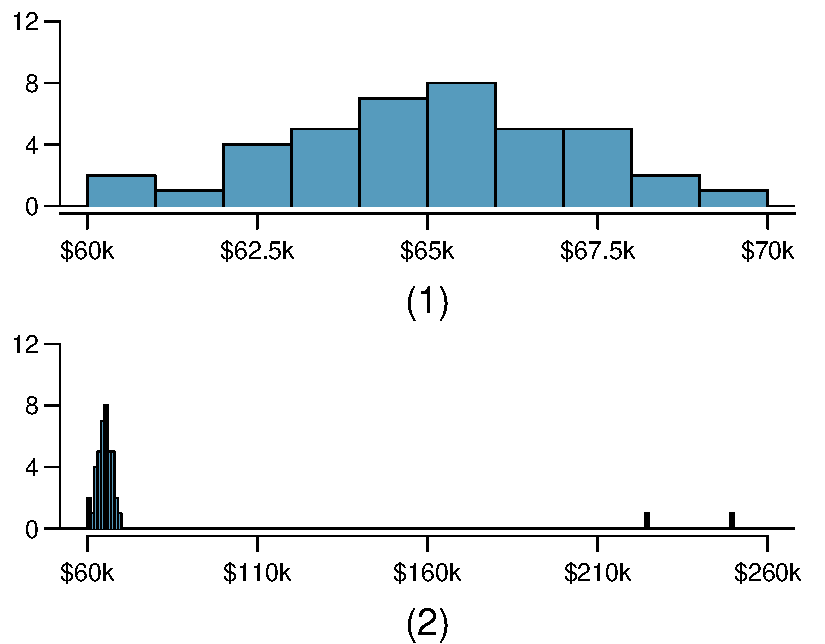
\includegraphics[scale=0.3]{figure/income_coffee_shop.pdf}
\end{minipage}
\begin{minipage}[c]{0.49\textwidth}
\begin{center}
\scriptsize
\begin{tabular}{rrr}
\hline
        & (1)       & (2) \\ 
\hline
n       & 40        & 42 \\ 
Min.    & 60,680    & 60,680 \\ 
1st Qu. & 63,620    & 63,710 \\ 
Median  & 65,240    & 65,350 \\ 
Mean    & 65,090    & 73,300 \\ 
3rd Qu. & 66,160    & 66,540 \\ 
Max.    & 69,890    & 250,000 \\ 
SD      & 2,122     & 37,321 \\ 
\hline
\end{tabular}
\end{center}
\end{minipage}
\begin{enumerate}[(a)]
\item Would the mean or the median best represent what we might think of as a typical income for the 42 patrons at this coffee shop?
\vspace{0.5cm}
\item Would the standard deviation or the IQR best represent the amount of variability in the incomes of the 42 patrons at this coffee shop? 
\vspace{0.5cm}
\end{enumerate}
\end{frame}

\end{document}